\documentclass[11pt,a4paper]{article}
\usepackage[utf8]{inputenc}
\usepackage[T1]{fontenc}
\usepackage{amsmath,amssymb,amsthm}
\usepackage{geometry}
\usepackage{graphicx}
\usepackage{tikz}
\usetikzlibrary{shapes,arrows,positioning,fit,calc}
\usepackage{listings}
\usepackage{xcolor}
\usepackage{hyperref}
\usepackage{booktabs}
\usepackage{longtable}
\usepackage{enumitem}
\usepackage{fancyhdr}
\usepackage{titlesec}

\geometry{margin=1in}
\hypersetup{colorlinks=true,linkcolor=blue,urlcolor=blue,citecolor=blue}

\pagestyle{fancy}
\fancyhf{}
\rhead{BetterSys HFT Analysis}
\lhead{15M Up/Down Strategy \& Backtesting}
\cfoot{\thepage}

\definecolor{codegreen}{rgb}{0,0.6,0}
\definecolor{codegray}{rgb}{0.5,0.5,0.5}
\definecolor{codepurple}{rgb}{0.58,0,0.82}
\definecolor{backcolour}{rgb}{0.95,0.95,0.92}

\lstdefinestyle{rustcode}{
    backgroundcolor=\color{backcolour},
    commentstyle=\color{codegreen},
    keywordstyle=\color{codepurple},
    numberstyle=\tiny\color{codegray},
    stringstyle=\color{codegreen},
    basicstyle=\ttfamily\footnotesize,
    breaklines=true,
    numbers=left,
    numbersep=5pt,
    frame=single,
    tabsize=2
}

\lstset{style=rustcode}

\title{\textbf{15-Minute Up/Down HFT Strategy:\\Architecture Analysis \& Backtesting System Integration}\\[0.5em]\large BetterSys Technical Documentation}
\author{System Architecture Analysis}
\date{January 2026}

\begin{document}

\maketitle
\tableofcontents
\newpage

%==============================================================================
\section{Executive Summary}
%==============================================================================

This document provides a comprehensive architectural analysis of the 15-minute Up/Down high-frequency trading (HFT) strategy implemented within BetterSys, with particular focus on its integration with the \texttt{backtest\_v2} backtesting framework. The system is designed for trading Polymarket binary outcome markets that settle based on whether an underlying asset's price increases or decreases within a 15-minute window.

\subsection{Key Components}

\begin{enumerate}
    \item \textbf{FAST15M Live Engine}: Event-driven reactive trading system in \texttt{vault/fast15m\_reactive.rs}
    \item \textbf{Probability Model}: Driftless lognormal model in \texttt{vault/updown15m.rs}
    \item \textbf{Position Sizing}: Kelly Criterion implementation in \texttt{vault/kelly.rs}
    \item \textbf{Backtesting Framework}: Production-grade deterministic simulator in \texttt{backtest\_v2/}
\end{enumerate}

\subsection{Current Status}

\begin{itemize}
    \item \textbf{Live Trading}: Paper trading operational with \texttt{PaperExecutionAdapter}
    \item \textbf{Backtesting}: Full infrastructure exists but \textbf{15M strategy not integrated}
    \item \textbf{Data Contract}: Production-grade requires full L2 deltas (currently snapshot-only)
\end{itemize}

%==============================================================================
\section{FAST15M Live Strategy Architecture}
%==============================================================================

\subsection{Overview}

The FAST15M engine implements an event-driven architecture that reacts to real-time price updates from Binance via WebSocket. The target is sub-10ms tick-to-trade latency, replacing the original polling-based design.

\subsection{Core Data Flow}

\begin{center}
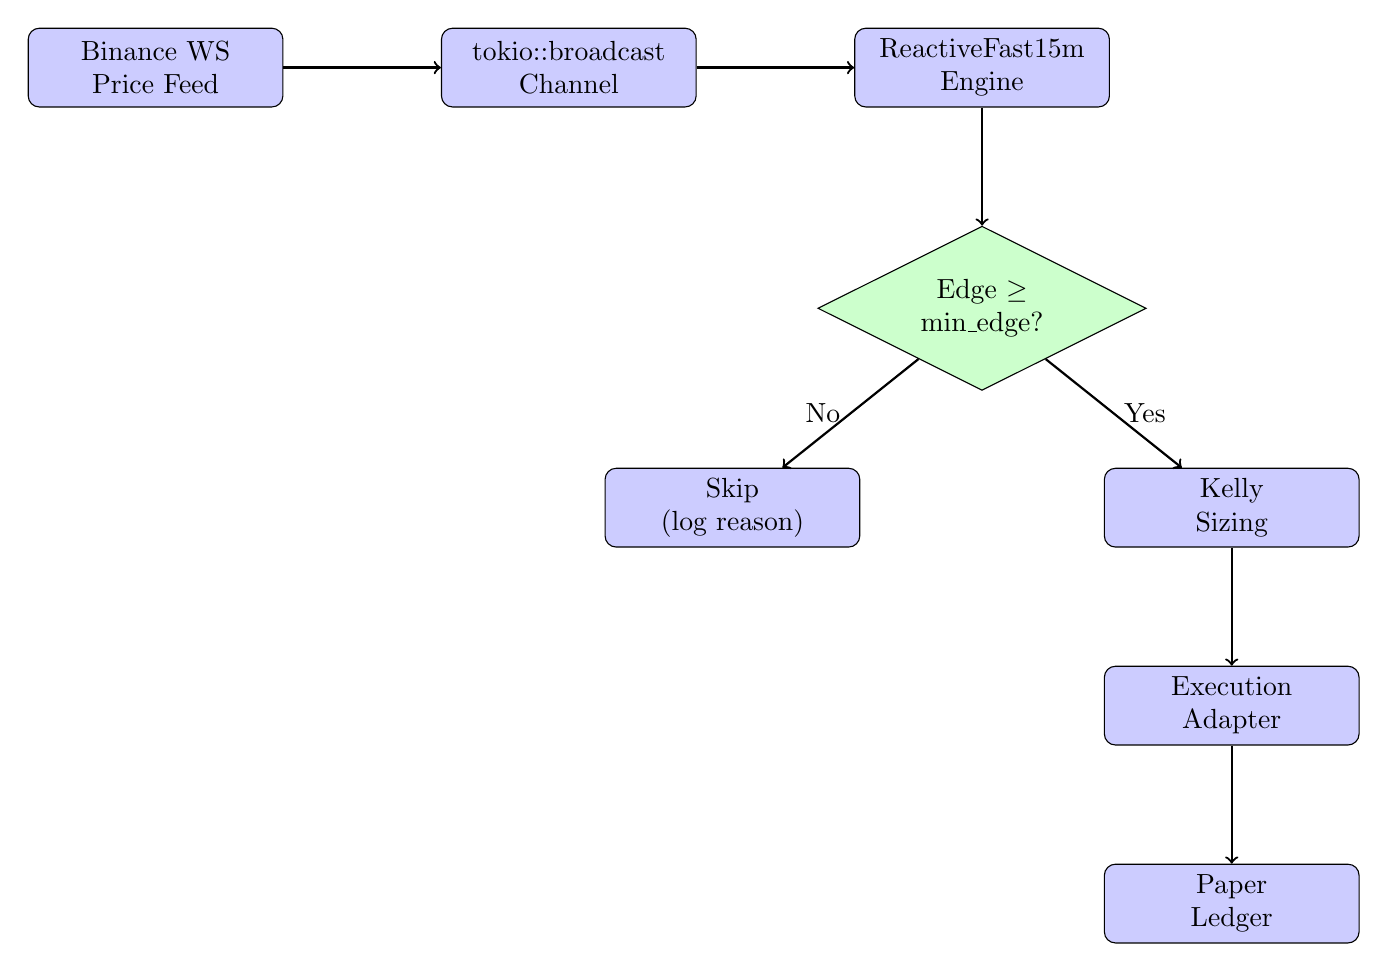
\begin{tikzpicture}[
    node distance=1.5cm,
    block/.style={rectangle, draw, fill=blue!20, text width=3cm, text centered, minimum height=1cm, rounded corners},
    decision/.style={diamond, draw, fill=green!20, text width=2cm, text centered, aspect=2},
    arrow/.style={->, thick}
]
    \node[block] (binance) {Binance WS\\Price Feed};
    \node[block, right=2cm of binance] (broadcast) {tokio::broadcast\\Channel};
    \node[block, right=2cm of broadcast] (engine) {ReactiveFast15m\\Engine};
    \node[decision, below=1.5cm of engine] (edge) {Edge $\geq$\\min\_edge?};
    \node[block, below left=1.5cm and 0.5cm of edge] (skip) {Skip\\(log reason)};
    \node[block, below right=1.5cm and 0.5cm of edge] (kelly) {Kelly\\Sizing};
    \node[block, below=1.5cm of kelly] (exec) {Execution\\Adapter};
    \node[block, below=1.5cm of exec] (ledger) {Paper\\Ledger};
    
    \draw[arrow] (binance) -- (broadcast);
    \draw[arrow] (broadcast) -- (engine);
    \draw[arrow] (engine) -- (edge);
    \draw[arrow] (edge) -- node[left] {No} (skip);
    \draw[arrow] (edge) -- node[right] {Yes} (kelly);
    \draw[arrow] (kelly) -- (exec);
    \draw[arrow] (exec) -- (ledger);
\end{tikzpicture}
\end{center}

\subsection{Probability Model}

The probability that the asset price ends \textbf{above} its starting price follows a driftless lognormal model:

\begin{equation}
P(\text{Up}) = \Phi\left(\frac{\ln(P_{\text{now}}/P_{\text{start}})}{\sigma\sqrt{t_{\text{rem}}}}\right)
\end{equation}

where:
\begin{itemize}
    \item $\Phi(\cdot)$ is the standard normal CDF
    \item $P_{\text{start}}$ is the price at window start
    \item $P_{\text{now}}$ is the current mid-price
    \item $\sigma$ is volatility per $\sqrt{\text{second}}$ (from Binance EMA)
    \item $t_{\text{rem}}$ is remaining seconds in the window
\end{itemize}

\subsection{Conservative Shrinkage}

To account for model uncertainty, the raw probability is shrunk toward 0.5:

\begin{equation}
P_{\text{adj}} = 0.5 + s \cdot (P_{\text{raw}} - 0.5), \quad s \in [0, 1]
\end{equation}

Default shrinkage factor $s = 0.35$ (configured via \texttt{UPDOWN15M\_SHRINK}).

\subsection{Kelly Position Sizing}

Position size is determined by fractional Kelly Criterion:

\begin{equation}
f^* = \frac{p \cdot b - q}{b}, \quad \text{where } b = \frac{1}{P_{\text{market}}} - 1
\end{equation}

Applied fractional Kelly:
\begin{equation}
f_{\text{actual}} = \min(f^* \cdot k_{\text{frac}}, f_{\text{max}}) \cdot \text{Bankroll}
\end{equation}

Default parameters:
\begin{itemize}
    \item $k_{\text{frac}} = 0.05$ (5\% of full Kelly)
    \item $f_{\text{max}} = 0.01$ (max 1\% of bankroll per trade)
    \item $\text{min\_position} = \$1$
\end{itemize}

\subsection{Latency Instrumentation}

The engine tracks detailed latency spans via \texttt{TradeSpan}:

\begin{table}[h]
\centering
\begin{tabular}{ll}
\toprule
\textbf{Stage} & \textbf{Description} \\
\midrule
\texttt{price\_received\_ns} & Timestamp when price update received \\
\texttt{evaluation\_start\_ns} & When strategy evaluation begins \\
\texttt{gamma\_lookup\_done\_ns} & After resolving Polymarket token IDs \\
\texttt{book\_fetch\_done\_ns} & After fetching orderbook (cache-only) \\
\texttt{kelly\_done\_ns} & After position sizing calculation \\
\texttt{order\_submitted\_ns} & When order sent to execution adapter \\
\texttt{order\_acked\_ns} & When execution confirmed \\
\texttt{ledger\_updated\_ns} & After ledger state updated \\
\bottomrule
\end{tabular}
\caption{Latency tracking stages in FAST15M engine}
\end{table}

%==============================================================================
\section{Backtesting Framework Architecture}
%==============================================================================

\subsection{Module Organization}

The \texttt{backtest\_v2} module comprises approximately 80+ Rust source files organized into functional subsystems:

\begin{center}
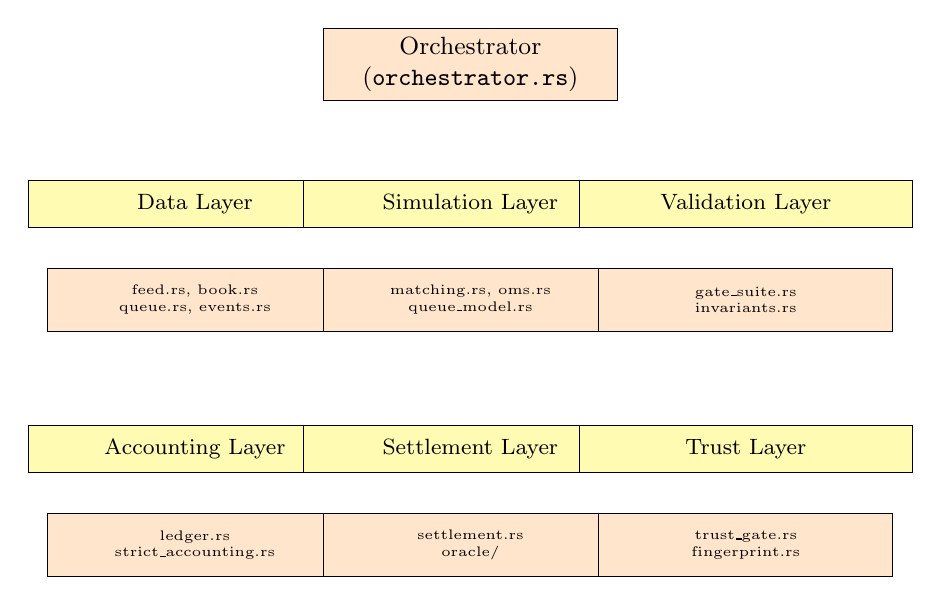
\begin{tikzpicture}[
    node distance=0.8cm,
    module/.style={rectangle, draw, fill=orange!20, text width=3.5cm, text centered, minimum height=0.8cm, font=\small},
    subsys/.style={rectangle, draw, fill=yellow!30, text width=4cm, text centered, minimum height=0.6cm, font=\footnotesize}
]
    \node[module] (orch) {Orchestrator\\(\texttt{orchestrator.rs})};
    
    \node[subsys, below left=1cm and -0.5cm of orch] (data) {Data Layer};
    \node[subsys, below=1cm of orch] (sim) {Simulation Layer};
    \node[subsys, below right=1cm and -0.5cm of orch] (val) {Validation Layer};
    
    \node[module, below=0.5cm of data, font=\tiny] (feed) {feed.rs, book.rs\\queue.rs, events.rs};
    \node[module, below=0.5cm of sim, font=\tiny] (match) {matching.rs, oms.rs\\queue\_model.rs};
    \node[module, below=0.5cm of val, font=\tiny] (gate) {gate\_suite.rs\\invariants.rs};
    
    \node[subsys, below=2.5cm of data] (acct) {Accounting Layer};
    \node[subsys, below=2.5cm of sim] (settle) {Settlement Layer};
    \node[subsys, below=2.5cm of val] (trust) {Trust Layer};
    
    \node[module, below=0.5cm of acct, font=\tiny] (ledger) {ledger.rs\\strict\_accounting.rs};
    \node[module, below=0.5cm of settle, font=\tiny] (settlem) {settlement.rs\\oracle/};
    \node[module, below=0.5cm of trust, font=\tiny] (trustm) {trust\_gate.rs\\fingerprint.rs};
\end{tikzpicture}
\end{center}

\subsection{Core Components}

\subsubsection{SimClock (\texttt{clock.rs})}

Monotonic nanosecond-precision simulation clock. All time references must use \texttt{SimClock::now()} - wall-clock access is forbidden via compile-time enforcement.

\begin{equation}
\text{Nanos} = i64 \quad (\text{nanoseconds since epoch})
\end{equation}

\subsubsection{Event Queue (\texttt{queue.rs})}

Priority queue with deterministic ordering:
\begin{equation}
\text{Order} = (\text{timestamp}, \text{priority}, \text{source}, \text{sequence})
\end{equation}

Events are processed in strict chronological order with tie-breaking by priority class (System $>$ BookSnapshot $>$ BookDelta $>$ TradePrint $>$ OrderAck $>$ Fill).

\subsubsection{Strategy Trait (\texttt{strategy.rs})}

The hermetic strategy interface:

\begin{lstlisting}[language=Rust]
pub trait Strategy: Send {
    fn on_book_update(&mut self, ctx: &mut StrategyContext, book: &BookSnapshot);
    fn on_trade(&mut self, ctx: &mut StrategyContext, trade: &TradePrint);
    fn on_timer(&mut self, ctx: &mut StrategyContext, timer: &TimerEvent);
    fn on_fill(&mut self, ctx: &mut StrategyContext, fill: &FillNotification);
    fn on_order_ack(&mut self, ctx: &mut StrategyContext, ack: &OrderAck);
    fn on_order_reject(&mut self, ctx: &mut StrategyContext, reject: &OrderReject);
    fn on_cancel_ack(&mut self, ctx: &mut StrategyContext, ack: &CancelAck);
    fn name(&self) -> &str;
}
\end{lstlisting}

\subsubsection{Matching Engine (\texttt{matching.rs})}

Full CLOB simulator with:
\begin{itemize}
    \item FIFO price-time priority
    \item Partial fills
    \item Self-trade prevention (4 modes)
    \item Configurable maker/taker fees
    \item Post-only order support
\end{itemize}

Price discretization to ticks:
\begin{equation}
\text{PriceTicks} = \text{round}\left(\frac{\text{price}}{\text{tick\_size}}\right), \quad \text{tick\_size} = 0.01
\end{equation}

\subsubsection{Queue Position Model (\texttt{queue\_model.rs})}

Tracks FIFO queue position for passive (maker) orders:

\begin{itemize}
    \item \textbf{size\_ahead}: Total shares ahead in queue
    \item \textbf{position}: Ordinal position (0 = front)
    \item \textbf{Cancel-fill race detection}: Compares cancel arrival time vs fill time
\end{itemize}

Fill probability estimation:
\begin{equation}
P(\text{fill}) = \min\left(1, \frac{V_{\text{expected}}}{\text{size\_ahead} + \text{our\_size}}\right)
\end{equation}

\subsection{Operating Modes}

The backtester automatically classifies runs into operating modes based on data contract:

\begin{table}[h]
\centering
\begin{tabular}{lll}
\toprule
\textbf{Mode} & \textbf{Data Requirement} & \textbf{Valid Claims} \\
\midrule
TakerOnly & Any orderbook & Taker PnL, signal timing \\
ResearchGrade & Snapshots + trades & Directional analysis \\
ProductionGrade & Full L2 deltas + seq & All claims including maker PnL \\
\bottomrule
\end{tabular}
\caption{Backtest operating modes}
\end{table}

\subsection{Data Contract Classification}

\begin{equation}
\text{DatasetClassification} = 
\begin{cases}
\text{FullIncremental} & \text{L2 deltas + exchange seq + trades} \\
\text{SnapshotOnly} & \text{Periodic snapshots} \\
\text{Incomplete} & \text{Missing orderbook or trades}
\end{cases}
\end{equation}

Queue modeling requires \texttt{FullIncremental}. The 15M strategy currently operates with \texttt{SnapshotOnly} data from periodic WS snapshots.

\subsection{Settlement Engine (\texttt{settlement.rs})}

First-class settlement modeling for 15M Up/Down markets:

\begin{lstlisting}[language=Rust]
pub struct SettlementSpec {
    window_duration_ns: 15 * 60 * NS_PER_SEC,  // 15 minutes
    reference_price_rule: ReferencePriceRule::MidPrice,
    tie_rule: TieRule::NoWins,  // tie => Down wins
    outcome_knowable_rule: OutcomeKnowableRule::OnReferenceArrival,
}
\end{lstlisting}

Outcome determination:
\begin{equation}
\text{Winner} = 
\begin{cases}
\text{Up (Yes)} & P_{\text{end}} > P_{\text{start}} \\
\text{Down (No)} & P_{\text{end}} \leq P_{\text{start}}
\end{cases}
\end{equation}

\subsection{Double-Entry Ledger (\texttt{ledger.rs})}

Production-grade accounting with:
\begin{itemize}
    \item Fixed-point arithmetic: $\text{Amount} = i128$, scale $= 10^8$
    \item Balanced entries: $\sum \text{debits} = \sum \text{credits}$
    \item Immutable append-only log
    \item Causal trace on violation
\end{itemize}

Account types:
\begin{itemize}
    \item \texttt{Cash}: USDC balance
    \item \texttt{CostBasis\{market, outcome\}}: Position cost basis
    \item \texttt{FeesPaid}: Accumulated fees
    \item \texttt{RealizedPnL}: Closed position P\&L
    \item \texttt{SettlementReceivable/Payable}: Settlement accounting
\end{itemize}

\subsection{Trust Gate (\texttt{trust\_gate.rs})}

Final arbiter of run validity. Trust decision requires:
\begin{enumerate}
    \item Production-grade config
    \item Settlement exact spec
    \item Ledger enforced (strict mode)
    \item Invariants hard mode
    \item Maker fills valid
    \item Data classification = FullIncremental
    \item Gate suite passed
    \item No sensitivity fragilities
\end{enumerate}

%==============================================================================
\section{Gap Analysis: Strategy-Backtest Integration}
%==============================================================================

\subsection{Critical Gap: No Backtest Strategy Implementation}

\textbf{The FAST15M live engine does not implement the \texttt{Strategy} trait and cannot be run in the backtester.}

The live engine (\texttt{ReactiveFast15mEngine}) is structured as:
\begin{itemize}
    \item Async event handler receiving \texttt{PriceUpdateEvent} via broadcast channel
    \item Direct access to \texttt{AppState} (HTTP client, WS caches, databases)
    \item Real-time token resolution via Gamma API
    \item Paper execution via \texttt{ExecutionAdapter}
\end{itemize}

The backtester requires:
\begin{itemize}
    \item Synchronous callbacks via \texttt{Strategy} trait
    \item Data access only through \texttt{StrategyContext} and \texttt{OrderSender}
    \item No external I/O (hermetic enforcement)
    \item Deterministic behavior (seeded RNG only)
\end{itemize}

\subsection{Data Contract Mismatch}

\begin{table}[h]
\centering
\begin{tabular}{lcc}
\toprule
\textbf{Feature} & \textbf{Live System} & \textbf{Backtest Requirement} \\
\midrule
Orderbook Updates & WS snapshots (periodic) & Full L2 deltas \\
Arrival Timestamps & Recorded at ingest & Required for visibility \\
Exchange Sequence & Not captured & Required for queue model \\
Trade Prints & \texttt{last\_trade\_price} WS & Full trade stream \\
\bottomrule
\end{tabular}
\caption{Data contract gap between live and backtest systems}
\end{table}

\subsection{Missing Components for Production Backtest}

\begin{enumerate}
    \item \textbf{Backtest Strategy Wrapper}: Translate \texttt{L2BookDelta} events to probability model inputs
    \item \textbf{Oracle Integration}: Binance price feed for settlement reference
    \item \textbf{Historical Data Pipeline}: Full incremental L2 deltas with sequence numbers
    \item \textbf{Strategy Factory Registration}: \texttt{make\_strategy("fast15m", params)}
\end{enumerate}

\subsection{Queue Model Applicability}

The 15M strategy is primarily a \textbf{taker} strategy (IOC/aggressive orders). Queue modeling is less critical but still relevant for:
\begin{itemize}
    \item Fill probability at current ask
    \item Slippage estimation
    \item Market impact analysis
\end{itemize}

Current implementation uses cache-only book fetches with skip-tick semantics on cache miss - this is \textbf{not reproducible} in backtest without recorded arrival times.

\subsection{Hermetic Violation Risks}

The live engine contains several hermetic violations:

\begin{lstlisting}[language=Rust]
// VIOLATION: Wall clock access
let now = Utc::now().timestamp();

// VIOLATION: External I/O
let up = polymarket_gamma::resolve_clob_token_id_by_slug(...).await?;

// VIOLATION: Shared mutable state
let bankroll = self.state.vault.ledger.lock().await.cash_usdc;
\end{lstlisting}

A backtest-compatible version must:
\begin{itemize}
    \item Use \texttt{ctx.timestamp} instead of \texttt{Utc::now()}
    \item Pre-resolve token IDs via \texttt{StrategyParams}
    \item Access positions via \texttt{ctx.orders.get\_position()}
\end{itemize}

%==============================================================================
\section{Proposed Integration Architecture}
%==============================================================================

\subsection{Strategy Adapter Pattern}

\begin{lstlisting}[language=Rust]
pub struct Fast15mBacktestStrategy {
    asset: UpDownAsset,
    cfg: ReactiveFast15mConfig,
    // Pre-resolved token IDs
    token_up: String,
    token_down: String,
    // State
    last_p_up: f64,
    last_trade_ts: Nanos,
    order_counter: u64,
}

impl Strategy for Fast15mBacktestStrategy {
    fn on_book_update(&mut self, ctx: &mut StrategyContext, book: &BookSnapshot) {
        // Extract mid price, compute p_up, evaluate edge, place order
    }
    
    fn on_fill(&mut self, ctx: &mut StrategyContext, fill: &FillNotification) {
        // Track fills for P&L
    }
    // ... other callbacks
}
\end{lstlisting}

\subsection{Data Requirements}

For production-grade backtesting, the data pipeline must provide:

\begin{enumerate}
    \item \textbf{Binance Mid-Price Feed}: For $P_{\text{start}}$, $P_{\text{now}}$, $\sigma$
    \item \textbf{Polymarket L2 Deltas}: For best ask at execution time
    \item \textbf{Recorded Arrival Times}: For visibility enforcement
    \item \textbf{Oracle Prices}: For settlement verification
\end{enumerate}

\subsection{Dual-Feed Architecture}

\begin{center}
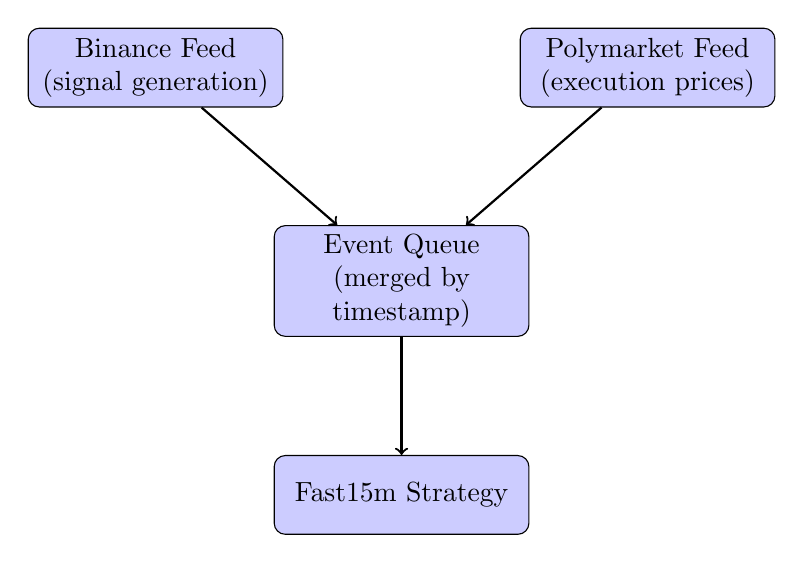
\begin{tikzpicture}[
    node distance=1.5cm,
    block/.style={rectangle, draw, fill=blue!20, text width=3cm, text centered, minimum height=1cm, rounded corners},
    arrow/.style={->, thick}
]
    \node[block] (binance) {Binance Feed\\(signal generation)};
    \node[block, right=3cm of binance] (poly) {Polymarket Feed\\(execution prices)};
    \node[block, below=2cm of $(binance)!0.5!(poly)$] (queue) {Event Queue\\(merged by timestamp)};
    \node[block, below=1.5cm of queue] (strat) {Fast15m Strategy};
    
    \draw[arrow] (binance) -- (queue);
    \draw[arrow] (poly) -- (queue);
    \draw[arrow] (queue) -- (strat);
\end{tikzpicture}
\end{center}

%==============================================================================
\section{Current Limitations Summary}
%==============================================================================

\begin{table}[h]
\centering
\begin{tabular}{p{4cm}p{4cm}p{4cm}}
\toprule
\textbf{Gap} & \textbf{Impact} & \textbf{Remediation} \\
\midrule
No \texttt{Strategy} impl & Cannot backtest 15M & Create adapter \\
Snapshot-only data & TakerOnly mode forced & Record L2 deltas \\
No exchange sequence & Queue model disabled & Add seq to recording \\
Hermetic violations & Non-deterministic results & Refactor for ctx-only \\
No Binance historical & Cannot reproduce $P_{\text{up}}$ & Record Binance mid \\
No Oracle integration & Settlement unverified & Add Chainlink feed \\
\bottomrule
\end{tabular}
\caption{Summary of integration gaps}
\end{table}

%==============================================================================
\section{Recommendations}
%==============================================================================

\subsection{Short-Term (TakerOnly Validation)}

\begin{enumerate}
    \item Create \texttt{Fast15mBacktestStrategy} implementing \texttt{Strategy} trait
    \item Use existing snapshot data with simulated latency
    \item Run in \texttt{TakerOnly} mode for directional validation
    \item Compare P\&L trajectory against paper trading logs
\end{enumerate}

\subsection{Medium-Term (Research-Grade)}

\begin{enumerate}
    \item Add \texttt{L2BookDelta} event recording to live ingestor
    \item Record Binance mid-prices with arrival timestamps
    \item Implement settlement verification against Chainlink
    \item Run sensitivity analysis on latency assumptions
\end{enumerate}

\subsection{Long-Term (Production-Grade)}

\begin{enumerate}
    \item Full L2 delta stream with exchange sequence numbers
    \item Queue model validation against realized fill rates
    \item Maker strategy extension (post-only quotes)
    \item Multi-asset correlation analysis
\end{enumerate}

%==============================================================================
\section{Conclusion}
%==============================================================================

The BetterSys backtesting framework (\texttt{backtest\_v2}) represents a sophisticated, production-grade simulation environment with comprehensive support for:

\begin{itemize}
    \item Deterministic replay with hermetic strategy enforcement
    \item Queue position modeling for maker strategies
    \item Double-entry accounting with strict invariants
    \item Settlement modeling with oracle integration
    \item Trust-gated result certification
\end{itemize}

However, the FAST15M live trading strategy is \textbf{not currently integrated} with this framework. The primary gaps are:

\begin{enumerate}
    \item Absence of a \texttt{Strategy}-compliant adapter
    \item Insufficient data fidelity (snapshots vs. deltas)
    \item Hermetic boundary violations in the live engine
\end{enumerate}

Addressing these gaps would enable rigorous historical validation of the 15M Up/Down strategy before live deployment with real capital.

\appendix

%==============================================================================
\section{Kelly Criterion Derivation}
%==============================================================================

For a binary outcome with probability $p$ of winning and decimal odds $b$:

\begin{align}
f^* &= \frac{p \cdot b - q}{b} \\
    &= \frac{p \cdot b - (1-p)}{b} \\
    &= p - \frac{1-p}{b}
\end{align}

For Polymarket where we buy at price $P$:
\begin{equation}
b = \frac{1}{P} - 1 = \frac{1-P}{P}
\end{equation}

Substituting:
\begin{equation}
f^* = p - \frac{(1-p) \cdot P}{1-P}
\end{equation}

When edge $= p - P > 0$:
\begin{equation}
f^* = \frac{\text{edge}}{1-P}
\end{equation}

%==============================================================================
\section{Driftless Lognormal Model}
%==============================================================================

Under the risk-neutral measure with zero drift, the log-return is:
\begin{equation}
\ln\left(\frac{S_T}{S_0}\right) \sim \mathcal{N}\left(-\frac{\sigma^2 T}{2}, \sigma^2 T\right)
\end{equation}

For the probability $S_T > S_0$:
\begin{equation}
P(S_T > S_0) = P\left(\ln\frac{S_T}{S_0} > 0\right) = \Phi\left(\frac{0 + \frac{\sigma^2 T}{2}}{\sigma\sqrt{T}}\right) = \Phi\left(\frac{\sigma\sqrt{T}}{2}\right)
\end{equation}

However, given current price $S_t$ with $t < T$, the conditional probability becomes:
\begin{equation}
P(S_T > S_0 \mid S_t) = \Phi\left(\frac{\ln(S_t/S_0)}{\sigma\sqrt{T-t}}\right)
\end{equation}

This is the model used in \texttt{p\_up\_driftless\_lognormal()}.

\end{document}
